\documentclass{article}
\usepackage[utf8]{inputenc}
\usepackage{tikz}
\usetikzlibrary{positioning}
\usetikzlibrary{shapes}

\begin{document}

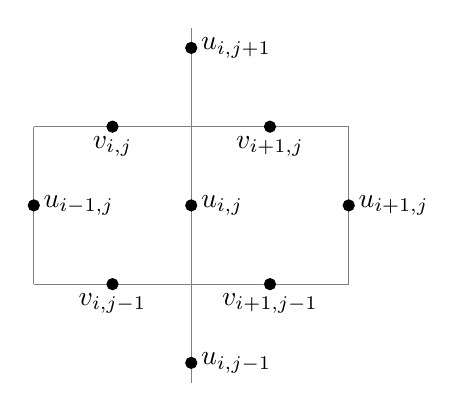
\begin{tikzpicture}
%grid
%horizontal
\draw[gray, thin] (-2,1) -- (2,1);
\draw[gray, thin] (-2,-1) -- (2,-1);
%vertical
\draw[gray, thin] (-2,1) -- (-2,-1);
\draw[gray, thin] (0,2.25) -- (0,-2.25);
\draw[gray, thin] (2,1) -- (2,-1);
%nodes
\filldraw [black] (0,0) circle (2pt) node[anchor=west] {$u_{i,j}$};
\filldraw [black] (0,2) circle (2pt) node[anchor=west] {$u_{i,j+1}$};
\filldraw [black] (2,0) circle (2pt) node[anchor=west] {$u_{i+1,j}$};
\filldraw [black] (0,-2) circle (2pt) node[anchor=west] {$u_{i,j-1}$};
\filldraw [black] (-2,0) circle (2pt) node[anchor=west] {$u_{i-1,j}$};
\filldraw [black] (1,1) circle (2pt) node[anchor=north] {$v_{i+1,j}$};
\filldraw [black] (1,-1) circle (2pt) node[anchor=north] {$v_{i+1,j-1}$};
\filldraw [black] (-1,-1) circle (2pt) node[anchor=north] {$v_{i,j-1}$};
\filldraw [black] (-1,1) circle (2pt) node[anchor=north] {$v_{i,j}$};

\end{tikzpicture}
\end{document}
